
\notesection{2023-12-22}{Tori, Pinnings, and Coherent Continuation}\label{1}

\subsection{Identification of co-character groups with Lie algebras}
Settings: $G$ complex connected reductive algebraic group. $Q \subseteq P \subseteq \fh^*$ are root lattice and weight group, respectively. $\check{Q} \subseteq \check{P} \subseteq \fh$ are coroot lattice and coweight group, respectively. $H$ is a maximal torus of $G$, $\fh$ is its Lie algebra.


There are identifications 
\defmap{I}{X_*(H)\otimes \BC}{\fh}{\phi}{\dd\phi\bra{1}}

\defmap{J}{X^*(H)\otimes \BC}{\fh ^*}{\varphi}{\dd \varphi}



Under these identifications we have

\begin{align*}
  P_* &= \bigset{\check{\lambda} \in \fh}{\bil{\alpha}{\check{\lambda}} \in \BZ, \textrm{for all $\alpha \in Q$}}\\
  & = \bigset{\check{\lambda} \in \fh}{\exp(2\pi\sqrt{-1}\bil{\alpha}{\check{\lambda}}) = 1, \textrm{for all $\alpha \in Q$}}\\
  & = \bigset{\check{\lambda} \in \fh}{\alpha(\exp(2\pi\sqrt{-1}\check{\lambda})) = 1, \textrm{for all $\alpha \in Q$}}\\
  & = \bigset{\check{\lambda} \in \fh}{\exp(2\pi\sqrt{-1}\check{\lambda}) \in Z(G)}.
\end{align*}
And
\begin{align*}
  X_{*}(H) & = \bigset{\check{\lambda} \in \fh}{\bil{\phi}{\check{\lambda}} \in \BZ, \textrm{for all $\phi \in X^*(H)$}}\\
  & = \bigset{\check{\lambda} \in \fh}{\exp(2\pi\sqrt{-1}\bil{\phi}{\check{\lambda}}) = 1, \textrm{for all $\phi \in X^*(H)$}}\\
  & = \bigset{\check{\lambda} \in \fh}{\phi(\exp(2\pi\sqrt{-1}\check{\lambda})) = 1, \textrm{for all $\phi \in X^*(H)$}}\\
  & = \bigset{\check{\lambda} \in \fh}{\exp(2\pi\sqrt{-1}\check{\lambda}) = 1}.
\end{align*} 

Similarly
$$P^* = \bigset{\lambda \in \fh^*}{\exp(2 \pi \sqrt{-1} \lambda) \in Z(\check{G})}. $$

$$X^*(H) = \bigset{\lambda \in \fh^*}{\exp(2 \ pi \sqrt{-1} \lambda ) = 1}.$$


Define $e: \fh \to H$ by $e(X) = \exp(2\pi\sqrt{-1}X)$, then $\ker(e) = X_*(H)$.

\[
\begin{tikzcd}
  \fh \arrow[r,"e"] & H \\
  P_* \arrow[r, "e"] \arrow[u,hook ] & Z(G) \arrow[u,hook]
\end{tikzcd}
\]

$Z(G) \simeq P_*/X_*(H)$.




\subsection{Pinnings of algebraic groups}

\begin{thm}[see \cite{AdC09}]
  Inner automorphism group $\mathrm{Inn(G)}$ of $G$ is equal to $\mathrm{G/Z(G)}$,
  $\mathrm{Inn(G)}$ acts freely and transitively on the set of pinnings.
\end{thm}


I know that there is an analogy in compact connected groups, and it has been proved.

\begin{thm}
  If $\RG$ is a compact connected group, then its inner automorphism group $\mathrm{Inn(G)} = \mathrm{G/Z(G)}$
  acts freely and transitively on the set of pinnings.
  (where pinnings for it is a bit different from the complex case, that $(T, B_\BC,\mathcal{X})$
  is a pinning if $T$ is a maximal torus, $B_\BC$ a Borel of $G_\BC$ containing $T$, $\mathcal{X}$
  is a set of real rays in simple root space.)
\end{thm}

\begin{proof}
  Here's proof from mathoverflow \href{https://mathoverflow.net/questions/377981/classification-of-not-necessarily-connected-compact-lie-groups/378141#378141}{Lspise's answer}:
  \begin{figure}[H]
    \centering
    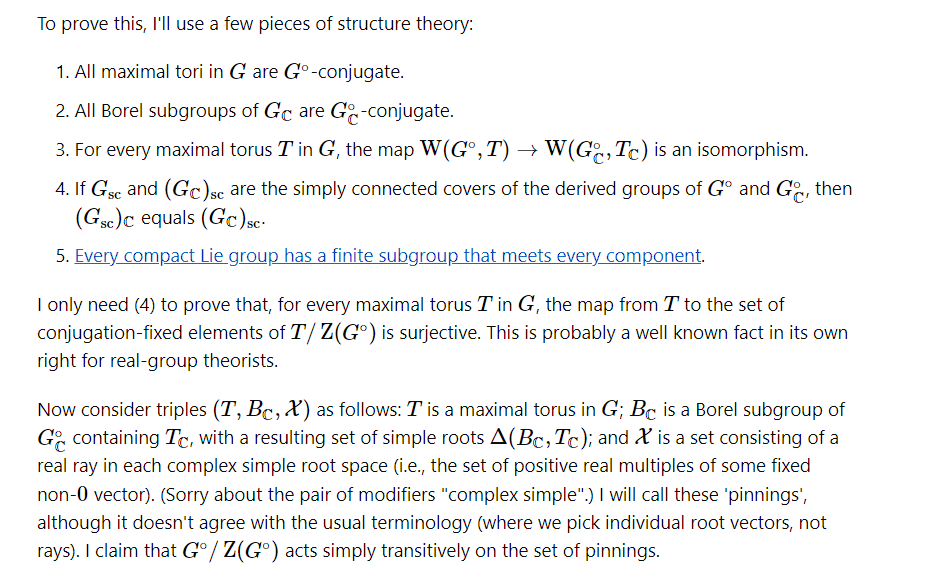
\includegraphics[width=1.0\linewidth]{1.png}
  \end{figure}

  \begin{figure}[H]
    \centering
    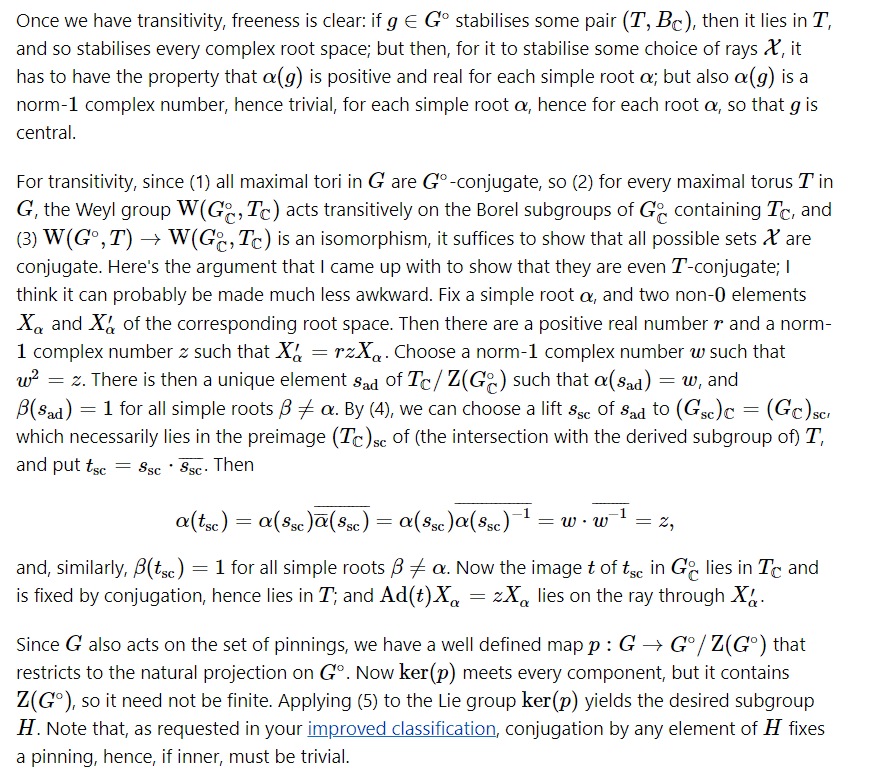
\includegraphics[width=1.0\linewidth]{2.png}
  \end{figure}
\end{proof}



\begin{rk}
  The pinnings show that split reductive algebraic groups look like butterflies!
\end{rk}

\begin{figure}[H]
  \centering
  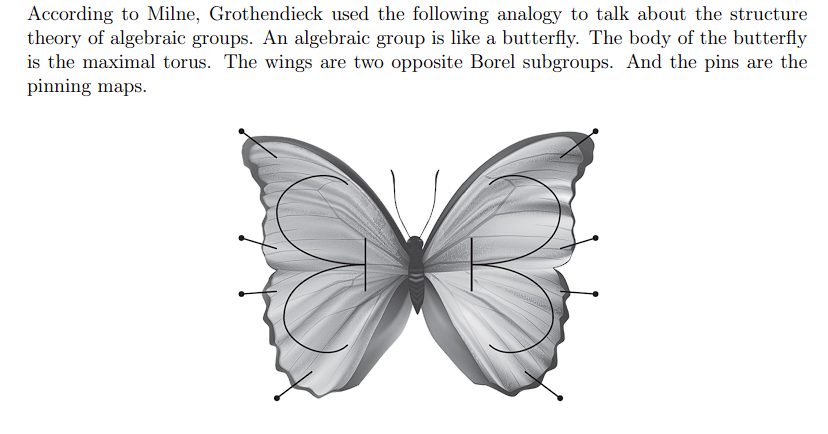
\includegraphics[width=1.0\linewidth]{3.png}
  \caption{Pinning of butterfly}
\end{figure}



\subsection{Coherent continuation representations}

Until the end of today, $G$ denotes a real reductive group in Harish-Chandra class.

Let's recall some basic definitions of coherent continuation representations, in order
for me to do calculations in the case of real classical groups.


Fix a connected reductive complex Lie group $G_\BC$, together with a Lie group homomorphism
$\iota: G \to  G_\BC$ such that its differential $\mathrm{d\iota} : \mathrm{Lie(G)} \to \mathrm{Lie(G_\BC)}$
has the following two properties:
\begin{enumerate}
  \item the kernel of $\mathrm{d\iota}$ is contained in the center of $\mathrm{Lie(G)}$;
  \item the image of $\mathrm{d\iota}$ is a real form of $\mathrm{Lie(G)}$.
\end{enumerate}

The analytical weight lattice of $\mathrm{G_\BC}$ is identified with a subgroup of $^{a}\fh^*$ via $\mathrm{d\iota}$.
We write $Q_\iota \subset \  ^{a}\fh^*$ for this subgroup. Denote root lattice by $Q_\fg$,
weight lattice by $Q^\fg$, then $$Q_\fg \subset Q_\iota \subset Q^\fg.$$
They are all $W$ stable subgroups.
And we have some categories:
\begin{enumerate}
  \item $\mathrm{Rep}(\fg,Q_\iota)$ the category of all finite-dimensional representations of $\fg$ whose weight are contained in $Q_\fg$, \textcolor{AttentionColor}{it can be identified with $\mathrm{Rep(Lie(G_\BC),Q_\iota)}$ and hence $\mathrm{Rep_{finite}(G_\BC)}$};
  \item $\mathrm{Rep(G)}$ the category of all Casselman-Wallach representations of $G$, and its full subcategories $\mathrm{Rep_\mu(G)}$, $\mathrm{Rep_S(G)}$.
\end{enumerate}
To denote their Grothendieck groups, we replace $\mathrm{Rep}$ by $\mathcal{K}$.


Fix a $Q_\iota$-coset $\Lambda = \lambda + Q_\iota \subset \  ^{a}\fh^*$.


\begin{defn}[coherent family]
  A $\mathcal{K}(G)$-valued $\Lambda$ coherent family is a map
  $$\varPhi : \Lambda \to \mathcal{K}(G)$$
  satisfies the following two conditions:
  \begin{enumerate}
    \item for all $\nu \in \Lambda$, $\varPhi(\nu) \in \mathcal{K}_{\nu}(G)$;
    \item for all representations $F \mathrm{ \in Rep}(\fg,Q_\iota)$ and all $\nu \in \Lambda$,
          $$F \cdot (\varPhi(\nu)) = \sum\limits_{\mu} \varPhi(\nu + \mu),$$
          where $\mu$ runs over all weights of $\mathrm{F}$, counted with multiplicities.
  \end{enumerate}
  The set of coherent families is denoted by $\mathrm{Coh}_\Lambda(\mathcal{K}(G))$
\end{defn}
We have the integral Weyl group $W_{\Lambda} = \set{w \in W}{w\lambda - \lambda \in Q_\iota}$
there is a representation of $W_\Lambda$ on $\mathrm{Coh}_\Lambda(\mathcal{K}(G))$ by
$$(w \cdot \varPhi)(\nu) = \varPhi (w^{-1}\nu).$$
This is called a coherent continuation representation.




\notesection{2023-12-23}{Regular Parameters and Outer Automorphisms}\label{2}

\subsection{Review of regular parameter}

Following yesterday's discussion of coherent continuation representations, we define two basis
for it, use Langland classification, follow \cite{BMSZ22}.

Suppose $H$ is a Cartan subgroup of $G$, by which we mean a subgroup that is the centralizer of
a Cartan subalgebra of $\Lie(G)$ \textcolor{ClarificationColor}{(In the case of linear groups, it's just a
  real algebraic torus.)}. $H$ has a unique maximal compact subgroup (since $G$ is in Harish-Chandra's
class, adjoint representation of $H$ is trivial, $H_0$ lies in the center of $H$, as we know, all
maximal subgroups of Lie groups are conjugate to each other, use Cartan decomposition of $H$, we win. In fact,
$H$ has a unique maximal compact torus and a unique maximal split torus)
We denote by $\Delta_{\fh} \subset \fh^*$ the root system of $\fg$. A root is called imaginary
if $\check{\alpha } \in \ft$ (i.e. roots which take pure imaginary values on $\Lie(H)$), an imaginary root $\alpha$ is
called compact if $\fg_{\alpha}$ and $\fg_{-\alpha}$ is contained in the complexified Lie algebra of a common compact subgroup of $G$.(this is equivalent to $\fg_\alpha $ belong to a Lie subalgebra of a compact subgroup, since $\fg_\alpha $ lies in a Lie subalgebra of maximal compact subgroup is equivalent to $\fg_{-\alpha }$ Lies in the same subgroup)


There are two important facts about the representation theory of $H$:
\begin{enumerate}
  \item Every Casselman-Wallach representation of $H$ is finite-dimensional, it follows directly from that $H$ is an extension of an abelian group and a finite group;
  \item For every $\Gamma \in \mathrm{Irr(H)}$ differential of $\Gamma$ is a direct sum of one-dimensional representations attached to a unique $\mathrm{d\Gamma \in \fh^*}$.
        (it is true because $H$ is in Harish-Chandra's class).
\end{enumerate}


For every Borel subalgebra $\fb$ of $\fg$ containing $\fh$, write 
$$\xi_{\fb}: \fh \to \ ^{a}\fh,$$
for the linear isomorphism attached to $\fb$ defined by 
$$\fh \hookrightarrow  \fb \to \fb / \sqbra{\fb,\fb} = \ {^{a}\fh}.$$
The transpose inverse of this map is still denoted by $\xi_{\fb}: \ ^{a}\fh^* \to \fh^*$.\\


Write $$W\bra{^{a}\fh^*,\fh^*} :=  \set{\xi_{\fb}: \ ^{a}\fh^* \to \fh^*}{\fb \ \textrm{is a Borel subalgebra containing} \ \fh}.$$

\begin{defn}
  For every element $\xi \in W\bra{^{a}\fh^*,\fh^*}$, put
  $$\delta(\xi) := \frac{1}{2} \cdot \sum\limits_{\alpha  \ \textrm{is an imaginary root in} \ \xi\Delta^+}\alpha - \sum\limits_{\beta \ \textrm{is an compact imaginary root in} \ \xi\Delta^+}\beta \in \fh^* .$$
  Write $\mathcal{P} _{\Lambda}(G)$ for the set of all triples $\gamma = (H,\xi,\Gamma)$, where
  $H$ is a Cartan subgroup of $G$, $\xi \in W\bra{^{a}\fh^*,\fh^*}$, and
  \defmap{\Gamma}{\Lambda}{\Irr(H)}{\nu}{\Gamma_{\nu}}
  is a map with the following properties:
  \begin{enumerate}
    \item $\Gamma_{\nu+\beta} = \Gamma_{\nu} \otimes \xi(\beta)$ for all $\beta \in Q_{\iota}$ and $\nu \in \Lambda$;
    \item $\mathrm{d\Gamma_{\nu}} = \xi(\nu) + \delta(\xi)$ for all $\nu \in \Lambda$.\textcolor{NoteColor}{(note that Cartan subgroups not always have irr repn with this differential!)}
  \end{enumerate}
  Here $\xi(\beta)$ is naturally viewed as a character of $H$ by using the homomorphism
  $\iota : H \to H_{\BC}$, and $H_{\BC}$ is a Cartan subgroup of $G_{\BC}$ containing $\iota(H)$.
\end{defn}



\subsection{Outer automorphism of algebraic groups}

\begin{lem}[a simple discover of abstract algebra]
  $G$ an abstract group, $H$ a normal subgroup of $G$, if $G$ acts
  transitively on a set $X$ such that the restriction of this action
  to $H$ is free and transitive, then the short exact sequence of groups
  $$\shortexact{1}{H}{G}{G/H}{1}$$
\end{lem}

\begin{proof}
  Actually choose an element $x \in X$, we have
  $$ G \simeq \mathrm{Stab}_{G}(x) \ltimes H.$$
\end{proof}


Using this lemma, we can see that for a complex connected reductive
algebraic group $G$, $\Aut(G)$ acts on the set of pinnings transitively,
with its normal subgroup the $\Inn(G)$ acts freely and transitively,
so every pinning gives us a split of the short exact sequence
$$\shortexact{1}{\Inn(G)}{\Aut(G)}{\Out(G)}{1}.$$


Some facts about split connected reductive algebraic groups over arbitrary field $k$:
\begin{enumerate}
  \item $\{ \textrm{split connected reductive algebraic groups} \}/_\backsim \ = \{ \textrm{root datums}\} /_\backsim $;
  \item For any two automorphisms of $G$, if they induce the same automorphism of root datum, then they differ by an inner automorphism;
  \item Fix a pinning, we get an isomorphism $\Out(G) \simeq \Aut(D_b)$.
\end{enumerate}


